\documentclass{article}
\usepackage{../../fasy-hw}

\title{Computational Geometry, Homework \hwnum}
\collab{n/a}

%% Instructor: update these macros:
\renewcommand{\hwnum}{5}
\date{due: Tuesday, 25 April 2023}

%% Student: update this macro:
\author{\todo{Your Name Here}}

\begin{document}

\maketitle

This homework assignment should be
submitted as a single PDF file to D2L.

General homework expectations:
\begin{itemize}
    \item Homework should be typeset using LaTex.
    \item Answers should be in complete sentences and proofread so that they
        make sense without seeing the question.
    \item You will not plagiarize, nor will you share your written solutions
        with classmates. (But, discussing the questions is highly encouraged).
    \item List collaborators at the start of each question using the
        \texttt{collab} command.
    \item Put your answers where the \texttt{todo} command currently is (and
        remove the \texttt{todo} macro, but not the word \texttt{Answer}).
    \item If you are asked to come up with an algorithm, you are
        expected to give an efficient algorithm (brute-force solutions will not
        be accepted). With your algorithm, please provide the following:
        \begin{itemize}
            \item \emph{What}: A prose explanation of the problem and the algorithm,
                including a description of the input/output.  Be sure to state
                your GP assumptions.
            \item \emph{How}: Describe how the algorithm works clearly.
                Including pseudocode may helpful.
            \item \emph{How Fast}: Runtime, along with the derivation.  (Or, at
                the very least, a proof of termination using a decrementing
                function).  You only need to specify the space complexity if the
                problem asks for it.
           \item \emph{Why}: Brief justification of why the algorithm works.
               Often, this will include a statement of the loop invariant for each
               (outer-most) loop, or recursion invariant for each recursive function.
        \end{itemize}
\end{itemize}

{\bf David Mount's tips for writing up homework solutions}:
Remember that your description is intended to be read by a
human, not a compiler, so conciseness and clarity are preferred over technical
details.  Unless otherwise stated, you may use any results from class, or
results from any standard textbook on algorithms and data structures. Also, you
may use results from geometry that: (1) have been mentioned in class, (2) would
be known to someone who knows basic geometry or linear algebra, or (3) is
intuitively obvious. If you are unsure, please feel free to check with me.

Giving careful and rigorous proofs can be quite cumbersome in geometry, and so
you are encouraged to use intuition and give illustrations whenever appropriate.
Beware, however, that a poorly drawn figure can make certain erroneous
hypotheses appear to be ``obviously correct.''

Throughout the semester, unless otherwise stated, you may assume that input
objects are in general position. For example, you may assume that no two points
have the same x-coordinate, no three points are collinear, no four points are
co-circular. Also, unless otherwise stated, you may assume that any geometric
primitive involving a constant number of objects each of constant complexity can
be computed in $\Theta(1)$ time


{\bf Acknowledgement}: the homework problems were adapted from assignments of David
Millman, which, in turn, were adaptations of problems by David Mount and Carola
Wenk.

%%%%%%%%%%%%%%%%%%%%%%%%%%%%%%%%%%%%%%%%%%%%%%%%%%%%%%%%%%%%%%%%%%%%%%%%%%%%%%
\collab{\todo{}}
\nextprob{Topological Sweep}

Suppose that we have a set of non-vertical lines $\mathcal{L}$ in general position (no two
parallel, and no three through a common point), and a ``vertical'' path $p$ that crosses each
line exactly once as they go from left-to-right. By this, we mean
that if we orient the lines in $\mathcal{L}$ from left to right, then the left
endpoints (at infinity) are to the left of $p$ and the right endpoints are to
the right of $p$.  Like \figref{arrangment} shows, this forces one endpoint
$p_0$ of
$p$ to be below all lines and the other endpoint $p_1$ to be above all lines.
Note that both $p_0$ and $p_1$ are points at infinity.  Think of $p$ as being
oriented from $p_0$ to $p_1$, so that when looking at intersections of lines
along $p$, we can talk about `above' and `below' (with respect to $p$).

The following steps
visit all intersections in this arrangement that are to the right of the path.

\begin{enumerate}[(a)]
    \item Define an \emph{upper horizon tree} (UHT) by starting with the rays defined
        by the lines of the
        arrangement starting at the path and towards the right. At each vertex where
        two rays collide, only the upper ray continues; continue clipping until
        every vertex of the UHT has two edges on left (between $p$ and the
        vertex) and one ray going to the right.
        The resulting UHT is
        shown in pink in
        \figref{arrangement}. Give an algorithm to
        compute the upper horizon tree in $O(n \log n)$ time.

        \todo{replace this TODO with your answer}

    \item Prove that if there are any arrangement vertices to the right of the
        path, then there is a triangle formed by the path and two edges of the
        upper horizon tree.  Prove also that the uppermost triangle (labeled
        $A$ in the \figref{arrangement}) is also a triangle of the arrangement.  (Note that
        the triangle labeled $B$ is not).

        \todo{replace this TODO with your answer}

    \item We can advance the path past the triangle so that the two edges swap
        order along the path.  Describe how to update the horizon tree to become
        the upper horizon tree for this modified path.

        \todo{replace this TODO with your answer}

    \item If we keep triangles in a stack from `left' to `right', we can always have
        access to the leftmost triangle.  How do we maintain this stack when we
        advance past a triangle?
        % Hint: need to define leftmost
        % Alt approach: use top/down ordering

        \todo{replace this TODO with your answer}

    \item Show that if we start the path as the line at infinity that intersects
        all lines to the right of all pairwise intersections, then
        the total time spent maintaining the upper horizon tree is
        $\Theta(n^2)$.  Hint: you can apply the Zone Theorem (Theorem 8.5 of the
        Dutch book) to each line in the arrangement.

        \todo{replace this TODO with your answer}

\end{enumerate}

Note: this HW assignment was borrowed from the Computational Geometry class that
I took at University of North Carolina with Jack Snoeyink.  Thanks, Jack!

\begin{figure}[bht]
    \centering
    \begin{subfigure}{.31\textwidth}
        \centering
        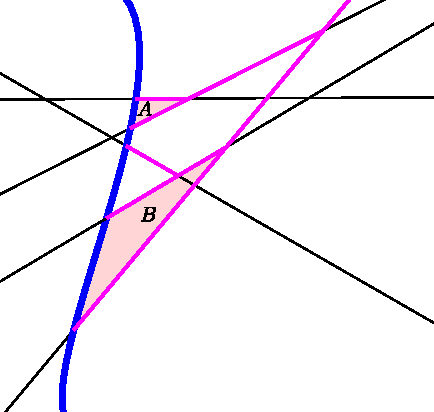
\includegraphics[width=\linewidth]{arrangement-before}
        \caption{Arrangement of five lines in the plane (black lines), and a path
            (bold~blue).}
        \label{fig:arrangement-before}
    \end{subfigure}
    ~
    \begin{subfigure}{.31\textwidth}
        \centering
        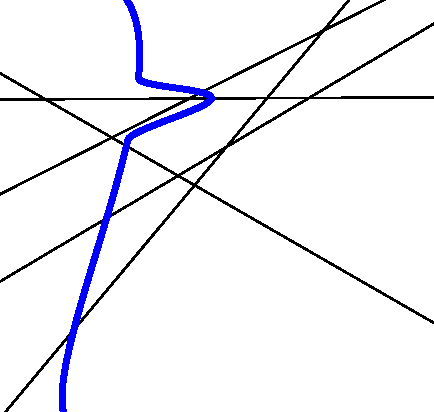
\includegraphics[width=\linewidth]{arrangement-after}
        \caption{After sweeping over a triangle. The only change is
        local, around the triangle swept over..}
        \label{fig:image-pixvert}
    \end{subfigure}
    \caption{Topologically sweeping an arrangement.}
    \label{fig:arrangement}
\end{figure}

%%%%%%%%%%%%%%%%%%%%%%%%%%%%%%%%%%%%%%%%%%%%%%%%%%%%%%%%%%%%%%%%%%%%%%%%%%%%%%

%%%%%%%%%%%%%%%%%%%%%%%%%%%%%%%%%%%%%%%%%%%%%%%%%%%%%%%%%%%%%%%%%%%%%%%%%%%%%%
\collab{\todo{}}
\nextprob{Reflection}

Explain to me anything that you tried differently on this homework, focused on
for improvement of technical writing, or what you would especially like feedback
on.  It can be something simple like ``Before this class, I was not very aware
of what tense I was writing in.  For this homework, I tried to focus on writing
in present tense.'' or something very focused, such as ``I really focused on
improving my End-condition proofs for loop invariants.''  If you tried something
and struggled, let me know. Since everyone needs to improve (including me),
there should be something that you can write about here.  You can base it on
feedback I gave you, feedback I gave the class, feedback you received from
someone else, an example of technical writing that you really liked, or anything
else that motivates you to improve.

\paragraph{Answer}

\todo{replace this TODO with your answer}
%%%%%%%%%%%%%%%%%%%%%%%%%%%%%%%%%%%%%%%%%%%%%%%%%%%%%%%%%%%%%%%%%%%%%%%%%%%%%%

\end{document}
